% ============================ 03 实验 ============================

\section{实验验证}

\begin{frame}[plain]
  \begin{center}
    \vspace{1.2cm}
    {\color{yopoblue}\Huge\bfseries 03}\\[0.5em]
    {\color{yopoblue}\LARGE 实验验证}\\[1.2em]
    \begin{minipage}{0.76\textwidth}
      \small\color{yopogray}
      本部分仅陈述原文可支持的结论及其边界。
      平台、密度、速度等前提均予保留，不同条件下的数字不直接比较。
    \end{minipage}
  \end{center}
\end{frame}

% ---------------------------------------------------------------
\begin{frame}{与梯度优化专家的对比}
  \small
  \begin{columns}[t]
    \begin{column}{0.56\textwidth}
      \begin{block}{原文表 I（PDF 第 6 页）}
        \footnotesize
        \begin{tabular}{@{}llrr@{}}
          \toprule
          方法 & 指标 & 代价 & 耗时 \\
          \midrule
          专家（50 步梯度下降） & 平均 & 0.078 & \multirow{2}{*}{30\,ms} \\
                                & 最优 & 0.036 & \\
          \addlinespace
          网络（初始） & 平均 & 0.105 & \multirow{4}{*}{1.6\,ms} \\
          网络（初始） & 最优 & 0.056 & \\
          网络（训练后） & 平均 & \textbf{0.050} & \\
          网络（训练后） & 最优 & \textbf{0.036} & \\
          \bottomrule
        \end{tabular}
      \end{block}
      \begin{reading}[“专家”的含义]
        \scriptsize
        指同一代价函数下的\textbf{经典梯度下降优化器}，
        从基元初值出发迭代 50 步。
        它是模仿学习里“提供示范”的那个上界，而不是 YOPO 训练的一部分。
      \end{reading}
    \end{column}
    \begin{column}{0.42\textwidth}
      \begin{reading}[结论适用范围]
        \small
        \begin{itemize}\tight
          \item 网络学到了有效的\textbf{快速映射}：
                耗时降低一个数量级以上；
          \item 在\textbf{平均候选代价}上优于所比较的专家；
          \item 最优候选代价与专家接近。
        \end{itemize}
      \end{reading}
      \begin{reading}[结论的边界]
        \small
        \begin{itemize}\tight
          \item 不能证明优于所有优化器；
          \item 不构成全局最优保证；
          \item 不能外推到未测试的初始条件分布。
        \end{itemize}
      \end{reading}
    \end{column}
  \end{columns}
\end{frame}

% ---------------------------------------------------------------
\begin{frame}{与 SOTA 方法对比：延迟、安全性与平滑性}
  \small
  \begin{center}\scriptsize
  \begin{tabular}{@{}lccccccc@{}}
    \toprule
    \multirow{2}{*}{方法} & 密度 & \multicolumn{4}{c}{延迟 / ms} &
    \multicolumn{2}{c}{障碍距离 / m} \\
    \cmidrule(lr){3-6}\cmidrule(lr){7-8}
     & (tree/m$^2$) & 建图 & 前端 & 后端 & \textbf{总计} & 平均 & 最小 \\
    \midrule
    \multirow{2}{*}{TopoTraj} & 1/30 & \multirow{2}{*}{48.5} & \multirow{2}{*}{6.1} & \multirow{2}{*}{7.3} & \multirow{2}{*}{61.9} & 1.23 & 0.18 \\
                              & 1/20 & & & & & 1.00 & 0.08 \\
    \addlinespace
    \multirow{2}{*}{MPPI} & 1/30 & \multirow{2}{*}{6.5} & \multirow{2}{*}{5.0} & \multirow{2}{*}{8.2} & \multirow{2}{*}{19.7} & 1.23 & 0.08 \\
                          & 1/20 & & & & & 0.94 & 0.06 \\
    \addlinespace
    \multirow{2}{*}{Agile Autonomy} & 1/30 & \multirow{2}{*}{/} & \multirow{2}{*}{/} & \multirow{2}{*}{/} & \multirow{2}{*}{5.4} & 1.13 & 0.12 \\
                                   & 1/20 & & & & & 1.01 & 0.10 \\
    \addlinespace
    \multirow{2}{*}{\textbf{YOPO}} & 1/30 & \multirow{2}{*}{/} & \multirow{2}{*}{/} & \multirow{2}{*}{/} & \multirow{2}{*}{\textbf{1.6}} & \textbf{1.63} & \textbf{0.24} \\
                                   & 1/20 & & & & & \textbf{1.28} & \textbf{0.16} \\
    \bottomrule
  \end{tabular}
  \end{center}
  \vspace{0.1em}
  \begin{reading}
    \footnotesize
    平台为 i7-9700 + RTX 3060，平均速度 4\,m/s。
    此设置下 YOPO 的\textbf{障碍间距最好}；
    但 MPPI 的\textbf{平滑性}更好（其平滑性代价 16.83\,m$^2$/s$^5$ 远低于 YOPO 的 73.52）。
    高速度、密集场景下 Agile Autonomy 更有竞争力——
    不能写成“YOPO 在所有速度和指标上都最优”。
  \end{reading}
\end{frame}

% ---------------------------------------------------------------
\begin{frame}{速度-成功率曲线与轨迹对比}
  \small
  \begin{columns}[c]
    \begin{column}{0.58\textwidth}
      \begin{tabular}{@{}cc@{}}
        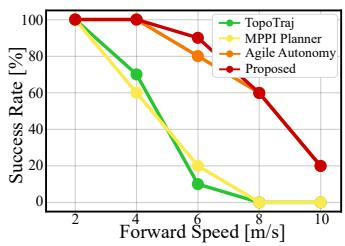
\includegraphics[width=0.47\linewidth]{figures/07a_success_sparse.jpg} &
        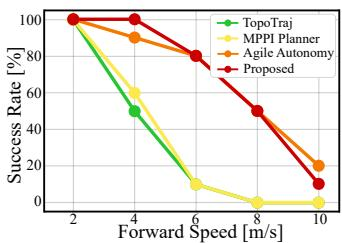
\includegraphics[width=0.47\linewidth]{figures/07b_success_dense.jpg}\\
        \scriptsize (a) 稀疏：1/30 tree/m$^2$ &
        \scriptsize (b) 密集：1/20 tree/m$^2$ \\
      \end{tabular}
      \begin{center}\scriptsize\color{yopogray}
      原文 Fig.~7：前飞速度 2--10\,m/s 的成功率，每个条件重复 10 次
      \end{center}
    \end{column}
    \begin{column}{0.4\textwidth}
      \footnotesize
      \begin{itemize}\tight
        \item 两种密度下，学习式方法的成功率\textbf{显著高于}经典视觉方法；
        \item 经典基线下降的原因：传感器量程有限、深度噪声、
              地图不完整；而概率式地图更新虽然能去噪，却让重建变慢；
        \item YOPO 在 \textbf{6\,m/s 以下}优于 Agile Autonomy，
              因为它并行预测更多拓扑不同的候选；
        \item 由于训练时考虑了平滑性，高速密集场景下会牺牲一部分安全性。
      \end{itemize}
    \end{column}
  \end{columns}
  \vspace{0.2em}
  \begin{center}
  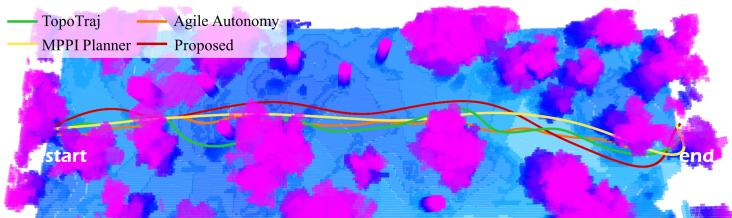
\includegraphics[width=0.46\linewidth]{figures/08a_trajectory_sparse.jpg}\hfill
  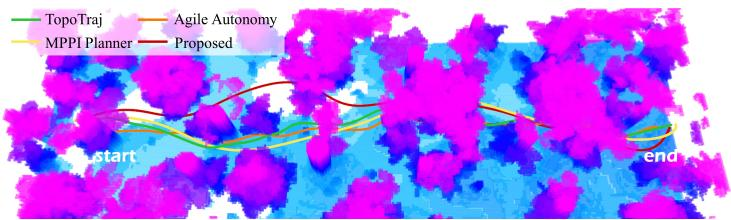
\includegraphics[width=0.46\linewidth]{figures/08b_trajectory_dense.jpg}
  \end{center}
  \begin{center}\scriptsize\color{yopogray}
  原文 Fig.~8：稀疏与密集森林中的轨迹对比
  \end{center}
\end{frame}

% ---------------------------------------------------------------
\begin{frame}{真机平台与机载配置}
  \small
  \begin{columns}[c]
    \begin{column}{0.5\textwidth}
      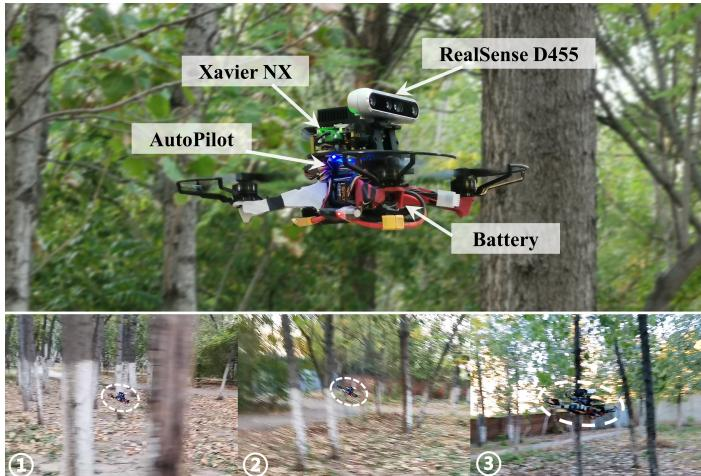
\includegraphics[width=\linewidth]{figures/09_platform.jpg}
      \begin{center}\scriptsize\color{yopogray}
      原文 Fig.~9：物理平台与真机实验场景
      \end{center}
    \end{column}
    \begin{column}{0.46\textwidth}
      \begin{block}{机载配置}
        \scriptsize
        \begin{itemize}\tight
          \item 250\,mm 轴距、1.13\,kg 四旋翼；
          \item RealSense D455 深度相机
                （$87^\circ\times58^\circ$，约 6\,m 量程）；
          \item VINS-Fusion 状态估计；
          \item Xavier NX 机载计算，TensorRT 部署后约 \textbf{16\,ms}；
          \item 几何控制器跟踪参考轨迹。
        \end{itemize}
      \end{block}
      \begin{reading}[相机与网络的衔接]
        \scriptsize
        真机图像宽高比 16:9，被缩放到 $160\times96$ 后输入网络；
        无效深度用最近邻插值填充，与训练时的处理保持一致。
      \end{reading}
    \end{column}
  \end{columns}
\end{frame}

% ---------------------------------------------------------------
\begin{frame}{真机飞行结果}
  \small
  \begin{center}
    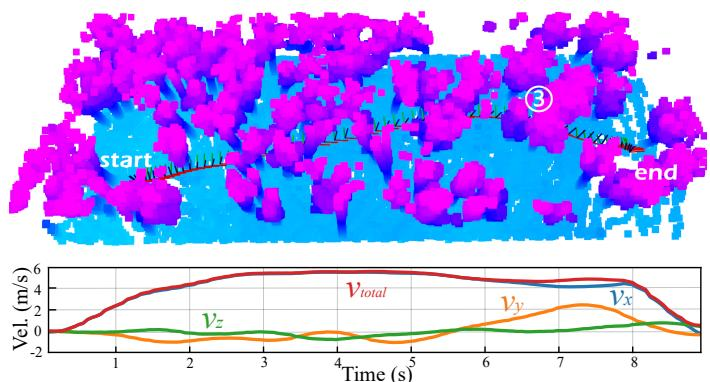
\includegraphics[width=0.66\linewidth]{figures/10c_map_and_velocity.jpg}
  \end{center}
  \vspace{-0.4em}
  \begin{center}\scriptsize\color{yopogray}
  原文 Fig.~10：真机飞行轨迹与速度曲线（地图仅用于展示，飞行中并不使用）
  \end{center}
  \vspace{0.2em}
  \begin{columns}[t]
    \begin{column}{0.48\textwidth}
      \begin{reading}[两个延迟指标的区分]
        \scriptsize
        桌面端 1.6\,ms 与机载 16\,ms 属于\textbf{不同平台}；
        二者都不能直接当作整条感知—规划—控制链路的端到端延迟。
      \end{reading}
    \end{column}
    \begin{column}{0.48\textwidth}
      \begin{reading}[飞行条件]
        \scriptsize
        最高速度 \textbf{5.52\,m/s}；实验森林密度 1/10 tree/m$^2$、
        树径约 0.25\,m；该环境在训练时\textbf{从未被观测过}。
      \end{reading}
    \end{column}
  \end{columns}
\end{frame}
